    \subsection{Benchmark Scope}
        The contribution of this work is the construction of a reproducible benchmark for a transparent MEA absorber model rather than the introduction of a new high-fidelity thermodynamic model. The same governing balances, reaction-enhancement model, transport-property correlations, and hydraulic calculations are used when comparing numerical solution methods and thermodynamic driving-force assumptions. The ePC-SAFT addition is not claimed as a new equation-of-state method; it is a read-only fugacity-coefficient lane inside the same benchmark. The primary ePC-SAFT comparison is neutral \COtwo--\MEA--\HtwoO{}, and a six-species ionic pressure-state lane is retained as diagnostic evidence using the current SSM/Born-enabled electrolyte contribution options. This framing makes each reported result traceable to a generated benchmark row that includes the case identifier, solver settings, initialization or scaling notes, thermodynamic model, convergence message, boundary residual, runtime, and validation error.

        The benchmark is therefore intended to answer three narrower questions. First, it evaluates how shooting, finite-difference, and SciPy collocation-style BVP solution paths behave when applied to the same column equations under both favorable one-bed and NCCC thermal-pinch conditions. Second, it evaluates how replacing the baseline Henry-law CO$_2$ fugacity driving force with ePC-SAFT fugacity-coefficient calculations changes capture predictions, temperature profiles, convergence, and runtime. Third, it tests whether explicit staged beds and liquid thermal resets can be represented without hiding solver failures. The benchmark should not be interpreted as evidence that the model is ready for industrial scale-up or process optimization without additional validation.

        The NCCC case labels are kept separate from the repository's legacy row identifiers. Morgan et al. label the Appendix C absorber temperature-profile cases as 1A--15A, 1B--3B, 1C--7C, and 1D--4D \cite{Morgan2020}. The separate 23-row staged capture benchmark used in the present repository is labeled K1--K23. Those K labels are treated as legacy capture-benchmark row identifiers, not as Appendix C case names. The one-bed C cases therefore support same-case temperature-profile validation, while the K rows support broader capture-rate and staged/intercooler solver diagnostics until a curated one-to-one Appendix C mapping is available.

    \subsection{Thermodynamic Driving-Force Comparison}
        The baseline thermodynamic lane uses the existing Henry-law calculation for the liquid CO$_2$ fugacity and an ideal vapor partial-pressure expression for the vapor fugacity. The ePC-SAFT lanes use the external ePC-SAFT package read-only and compute the CO$_2$ fugacity coefficient from pressure-specified phase states. The PC-SAFT and ePC-SAFT formulations are established equation-of-state approaches for associating and electrolyte-containing systems \cite{Gross2001,Cameretti2005}. PC-SAFT and SAFT-family parameters for CO$_2$ solubility in aqueous MEA have been reported by Fakouri Baygi and Pahlavanzadeh, Najafloo and Zarei, and Mac Dowell et al. \cite{Baygi2015,Najafloo2018,MacDowell2010}. Recent ePC-SAFT acid-gas and electrolyte studies provide additional context for EOS-based amine-solution calculations and for SSM/Born electrolyte contributions \cite{Cleeton2020,Bulow2021a,Schick2023,Rueben2024,Figiel2025}. The six-species ionic diagnostic lane uses the electrolyte contribution stack, including the Debye--Huckel and SSM/Born terms \cite{Bulow2020,Figiel2025}. In the present benchmark, ePC-SAFT is used as an EOS-based fugacity-coefficient lane for the CO$_2$ driving force. This comparison carries higher computational cost than Henry, so the expected direction is slower runtime, not faster runtime.

        In the present benchmark, only the CO$_2$ fugacity driving force is changed:
        \begin{align}
            f_{\COtwo}^{v} &= y_{\COtwo}\phi_{\COtwo}^{v}P,\\
            f_{\COtwo}^{\liq} &= x_{\COtwo}^{\liq}\phi_{\COtwo}^{\liq}P.
        \end{align}
        Chemical equilibrium, ionic speciation, enhancement factors, transport properties, heat-transfer correlations, and column balances are otherwise held fixed. The ePC-SAFT results are consequently reported as thermodynamic fugacity studies, not as full electrolyte-reactive ePC-SAFT MEA absorber models. The neutral lane uses a neutral-composition proxy. The ionic diagnostic lane uses the six true liquid species $\left(\COtwo,\MEA,\HtwoO,\MEAH,\MEACOO,\HCOthree\right)$ from the existing chemistry model, but does not replace that chemistry model. No speed claim is made against eNRTL in this manuscript; that comparison remains a future, unbenchmarked motivation.

        A diagnostic staged ePC-SAFT subset has also been generated for 19 selected legacy K rows. Thirteen of the 19 rows satisfy the strict success definition used here: solver success after post-processing gates, an eight-percentage-point capture-error gate, and a boundary residual norm below one. K2 collapses to the zero-capture branch under the nominal high-capture staged settings. K4, K9, and K19 are rejected by the capture-error gate, while K22 and K23 are rejected by the strict boundary-residual gate despite small capture errors. A targeted recovery probe covers K2, K4, K9, K19, and K23 using documented capture-initialization and intercooler-strength multistarts. That probe recovers K4, K9, and K23 with low boundary residuals, leaving K2 and K19 unresolved for the full neutral ePC-SAFT endpoint. K22 is retained as an unresolved boundary-residual diagnostic row in the current staged ePC-SAFT subset because it has not yet been accepted by a recovery artifact. A separate K2 fugacity-blend probe shows that partial Henry/ePC-SAFT blends recover the high-capture branch, while the full ePC-SAFT endpoint returns to the zero-capture branch under the same staged absorption-only setting. These rows are useful diagnostic evidence that the Henry-seeded staged ePC-SAFT pathway can run and emit cache/density-solve diagnostics, but they are not yet primary predictive validation.

    \subsection{Staged and Intercooled NCCC Cases}
        The single-bed validation is extended with an explicit staged-bed representation for the intercooled NCCC cases. In this configuration, each packed bed is represented by its own BVP segment. Vapor states are continuous upward from one bed to the next, while liquid states are continuous downward except at intercooler locations. Intercoolers are modeled as liquid thermal resets between adjacent packed beds. This treatment is consistent with the broader absorber heat-integration literature, where solvent cooling and heat-exchange packing alter the temperature profile and driving-force distribution \cite{Moore2021}. Morgan et al. reported that NCCC absorber temperature-profile shapes depend strongly on L/G ratio, lean loading, bed count, and solvent intercooling, and tabulated the Appendix C absorber profiles used here as an external qualitative check \cite{Morgan2020}. When measured inter-stage target temperatures or heat duties are unavailable for a specific benchmark row, the lean-solvent feed temperature is used as the liquid reset target and the benchmark row records this assumption. This is a first-order representation of solvent cooling, not a detailed intercooler plant model.

        This treatment is intentionally limited. It captures the first-order effect of solvent cooling on the downstream driving force, but it does not model detailed heat-exchanger approach temperatures, pressure losses through intercooler equipment, tray holdup, redistribution maldistribution, or measured heat duty. Those additions would require additional plant data and should be separated from the numerical and thermodynamic benchmark. The verified NCCC capture-rate evidence is therefore broader than a single-case demonstration but still partial: 19 of the 23 K cases are accepted as post-processing-gated capture-evidence rows under documented Henry-law staged/single-bed benchmark settings. These include cases with non-ideal solver status notes, such as low-residual final iterates or profile fallbacks, while excluded cases are handled in recovery or diagnostic artifacts. The remaining K6, K7, K8, and K20 cases also have separate diagnostic or sensitivity-recovery rows that fall within the capture-error gate under recovery settings, but those rows require high correction factors, suppressed intercooler strength, or large guard counts and are therefore not counted as primary predictive validation. The full staged ePC-SAFT lane likewise remains active benchmark work.

    \subsection{Generated Validation Metrics}
        The validation metrics below distinguish primary validation rows, accepted fallback rows, and diagnostic or recovery rows. This distinction matters because not every row that produces a plausible capture value is counted as primary validation. Rows requiring case-specific recovery settings are retained as diagnostic evidence, while rows used for stronger validation claims must satisfy the documented post-processing gates without hiding solver status, boundary residuals, profile caveats, or the no-case-specific-tuning gate.

        Table~\ref{tab:validation-evidence-registry} summarizes the evidence classes used in the revised benchmark. The one-bed C-case rows are clean primary validation rows for both thermodynamic lanes. The staged Henry legacy K-row table is broader and more useful for absorber operating-range coverage, but the accompanying no-case-specific-tuning gate shows that only part of the current staged table uses the same global continuation settings. The manuscript therefore treats the staged K rows as accepted validation evidence and reports the tuning gate explicitly instead of using them to claim complete predictive accuracy.

        \begin{table}
            \centering
            \scriptsize
            \caption{Evidence classes used by the NCCC validation artifacts. Diagnostic and recovery rows are retained in the repository but are not mixed into the strongest validation claims.}
            \label{tab:validation-evidence-registry}
            \renewcommand{\arraystretch}{1.2}
            \resizebox{\textwidth}{!}{%
            \begin{tabular}{lccccc}
                \toprule
                \textbf{Evidence group} & \textbf{Class} & \textbf{Rows} & \textbf{Accepted rows} & \textbf{Capture MAE (\%)} & \textbf{Median runtime (s)} \\
                \midrule
                One-bed C cases, Henry & Primary & 7 & 7 & 9.36 & 9.92 \\
                One-bed C cases, neutral ePC-SAFT & Primary & 7 & 7 & 9.37 & 27.63 \\
                Staged/intercooled K cases, Henry & Accepted validation & 19 & 19 & 2.82 & 7.78 \\
                K-case recovery rows, Henry & Recovery & 4 & 4 & 3.46 & 8.79 \\
                Staged K cases, neutral ePC-SAFT nominal & Diagnostic & 19 & 13 & 3.25 & 19.33 \\
                Staged K cases, neutral ePC-SAFT recovery & Recovery & 5 & 3 & 4.52 & 90.43 \\
                \bottomrule
            \end{tabular}%
            }
        \end{table}

        Table~\ref{tab:no-case-specific-tuning-gate} records the no-case-specific-tuning screen. The C-case groups pass this gate. The staged K-case table remains useful because it exposes the multi-bed/intercooler behavior and accepted capture rows, but the current staged evidence does not yet support a claim that one single global setting set reproduces all K cases. That limitation is part of the result.

        \begin{table}
            \centering
            \small
            \caption{No-case-specific-tuning gate for the accepted validation groups.}
            \label{tab:no-case-specific-tuning-gate}
            \renewcommand{\arraystretch}{1.2}
            \begin{tabular}{lccc}
                \toprule
                \textbf{Evidence group} & \textbf{Thermo model} & \textbf{Rows passing gate} & \textbf{Gate result} \\
                \midrule
                One-bed C cases & Henry & 7 of 7 & Pass \\
                One-bed C cases & Neutral ePC-SAFT & 7 of 7 & Pass \\
                Staged/intercooled K cases & Henry & 3 of 19 & Partial \\
                \bottomrule
            \end{tabular}
        \end{table}

        Table~\ref{tab:verified-one-bed-thermo-benchmark} summarizes the verified one-bed C-case thermodynamic benchmark computed from the verified C-case benchmark artifacts. Both thermodynamic lanes solved all seven one-bed cases in this artifact. The ePC-SAFT lane gives nearly the same aggregate capture error as the Henry-law lane, but it is slower in the median runtime because each residual evaluation requires ePC-SAFT fugacity-coefficient calculations. That runtime penalty is expected for the more explicit EOS lane and is part of the benchmark result, not a defect in the table.

        \begin{table}
            \centering
            \scriptsize
            \caption{Verified one-bed C-case benchmark summary for the Henry-law and neutral ePC-SAFT thermodynamic lanes.}
            \label{tab:verified-one-bed-thermo-benchmark}
            \renewcommand{\arraystretch}{1.2}
            \resizebox{\textwidth}{!}{%
            \begin{tabular}{lccccc}
                \toprule
                \textbf{Thermo model} & \textbf{Runs} & \textbf{Successes} & \textbf{Capture MAE, mean $|\epsilon_{\mathrm{cap}}|$ (\%)} & \textbf{Temp. RMSE (K)} & \textbf{Median runtime (s)} \\
                \midrule
                Henry-law baseline & 7 & 7 & 9.36 & 6.44 & 9.92 \\
                Neutral ePC-SAFT & 7 & 7 & 9.37 & 8.17 & 27.63 \\
                \bottomrule
            \end{tabular}%
            }
        \end{table}

        Table~\ref{tab:verified-staged-kcase-benchmark} reports the accepted legacy K-row capture-rate benchmark. The accepted rows include twelve three-bed/two-intercooler cases, one three-bed case without intercooling, two two-bed cases without intercooling, two two-bed/one-intercooler cases, and two one-bed cases. Across these 19 accepted rows, the mean absolute capture error is 2.81 percentage points and the maximum absolute error is 6.40 percentage points. Some accepted rows, including K13, use the temperature-only profile fallback after a transport-property profile diagnostic; those rows are accepted for capture-rate validation but should not be overinterpreted as full transport-profile validation. A separate sensitivity-recovery artifact records K6, K7, K8, and K20. Those rows demonstrate that all 23 K rows have at least one documented run below the eight-percentage-point capture screen, but the recovery rows are not treated as primary validation because K6 and K7 require a fivefold mass-transfer factor, K8 requires suppressing the intercooler reset, and K20 retains large guard counts and a mesh-limit status.

        \begin{table}
            \centering
            \small
            \caption{Verified legacy K-row capture-rate benchmark groups available for the Henry-law thermodynamic lane.}
            \label{tab:verified-staged-kcase-benchmark}
            \renewcommand{\arraystretch}{1.2}
            \begin{tabular}{lcccl}
                \toprule
                \textbf{Configuration} & \textbf{Accepted rows} & \textbf{Available rows} & \textbf{Capture MAE (\%)} & \textbf{Largest error (\%)} \\
                \midrule
                3 beds, 2 intercoolers & 12 & 15 & 3.53 & 6.40 \\
                3 beds, 0 intercoolers & 1 & 1 & 2.28 & 2.28 \\
                2 beds, 0 intercoolers & 2 & 2 & 1.45 & 2.74 \\
                2 beds, 1 intercooler & 2 & 2 & 0.77 & 1.20 \\
                1 bed, 0 intercoolers & 2 & 3 & 2.19 & 3.71 \\
                \midrule
                All accepted K rows & 19 & 23 & 2.81 & 6.40 \\
                \bottomrule
            \end{tabular}
        \end{table}

        Figure~\ref{fig:intercooled-temperature-profile-comparison} compares representative intercooled temperature behavior from the current model with measured NCCC absorber temperature data digitized from Appendix C of Morgan et al. \cite{Morgan2020}. The two panels are not the same operating point and are not used as a point-for-point validation metric. They are included to show that the staged/intercooled implementation can produce the same qualitative feature that appears in the NCCC profiles: a non-monotonic absorber temperature profile with cooling/reset behavior between packed sections. The measured NCCC data are plotted as unconnected markers to avoid implying interpolation between thermocouple locations.

        \begin{figure}
            \centering
            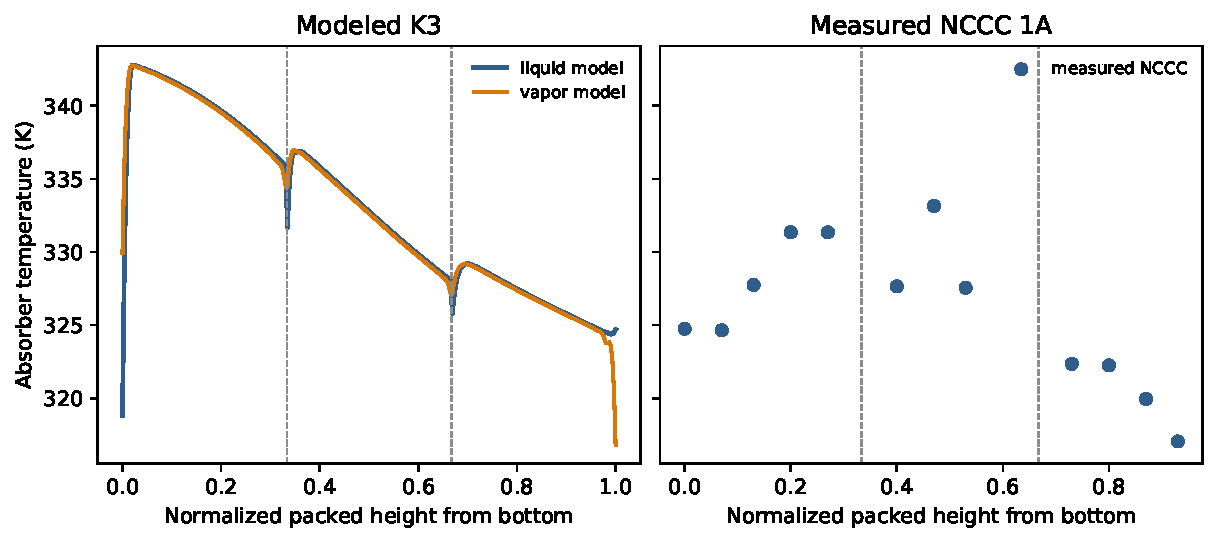
\includegraphics[width=0.92\textwidth]{figures/intercooled-temperature-profile-comparison.pdf}
            \caption{Representative intercooled absorber temperature behavior. The modeled legacy K3 row is shown as continuous liquid and vapor profiles from the solved BVP. The NCCC 1A measurements from Morgan et al. Appendix C are shown as unconnected markers because they are discrete temperature measurements and not an interpolated profile. The comparison is qualitative and supports the staged/intercooler behavior, not a direct same-case temperature RMSE claim.}
            \label{fig:intercooled-temperature-profile-comparison}
        \end{figure}

        Figure~\ref{fig:error-regime-capture-error} shows capture error against simple operating-regime descriptors. This plot is used to avoid a vague global predictive claim: the model is stronger for the accepted staged K capture rows than for the one-bed C thermodynamic sensitivity rows, and the largest one-bed C errors remain visible instead of being hidden by aggregate statistics.

        \begin{figure}
            \centering
            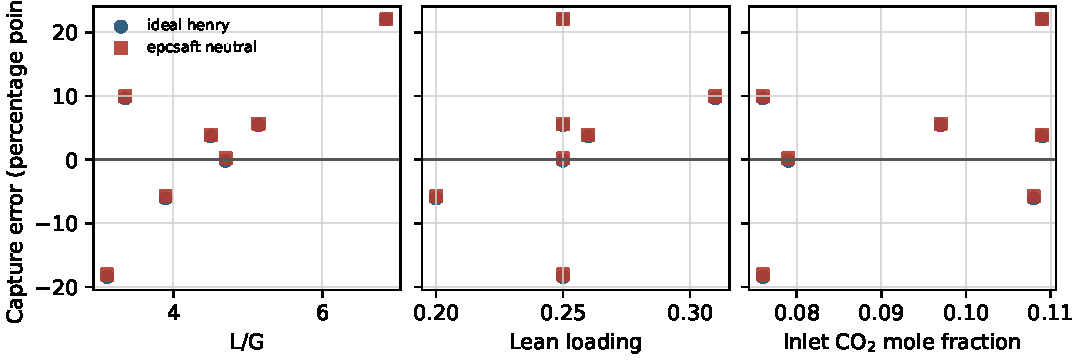
\includegraphics[width=0.92\textwidth]{figures/error-regime-capture-error.pdf}
            \caption{Capture error by operating-regime descriptors for the accepted Henry-law C and K validation rows. Dashed lines mark an eight-percentage-point capture-error screen used for staged K acceptance.}
            \label{fig:error-regime-capture-error}
        \end{figure}

        A small calibration screen was added as a low-cost credibility test rather than as a final tuned model. The screen uses the accepted K rows, splits the data by bed/intercooler pattern, and holds out the highest-numbered case in each pattern. A three-term global residual correction in $L/G$, lean loading, and inlet CO$_2$ mole fraction is fitted only on the training rows. Table~\ref{tab:calibration-holdout-screen} and Figure~\ref{fig:calibration-uncertainty-band} report the result. This screen improves the holdout capture MAE from 2.41 to 1.25 percentage points, but it is intentionally described as a residual-correction screen, not as a mechanistic refit of mass-transfer, heat-transfer, or intercooler parameters.

        \begin{table}
            \centering
            \small
            \caption{Structured holdout calibration screen for accepted staged K rows.}
            \label{tab:calibration-holdout-screen}
            \renewcommand{\arraystretch}{1.2}
            \begin{tabular}{lccccc}
                \toprule
                \textbf{Split} & \textbf{Cases} & \textbf{Raw MAE (\%)} & \textbf{Raw RMSE (\%)} & \textbf{Screened MAE (\%)} & \textbf{Screened RMSE (\%)} \\
                \midrule
                Training & 14 & 2.96 & 3.40 & 1.54 & 1.87 \\
                Holdout & 5 & 2.41 & 2.92 & 1.25 & 1.67 \\
                \bottomrule
            \end{tabular}
        \end{table}

        \begin{figure}
            \centering
            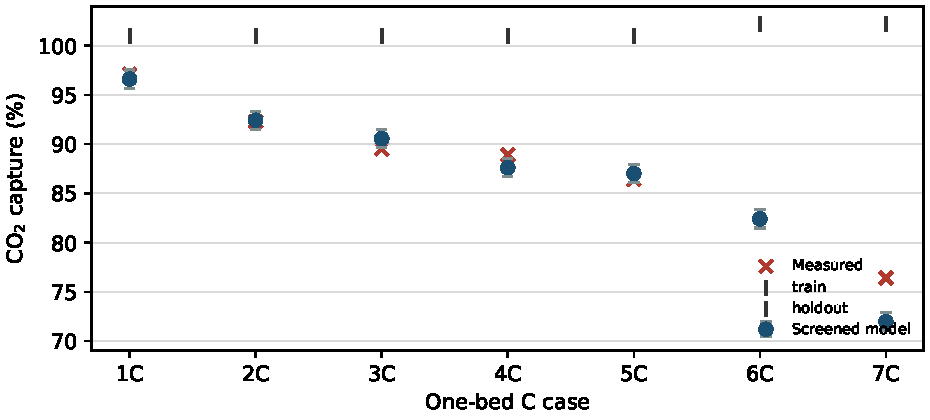
\includegraphics[width=0.86\textwidth]{figures/calibration-uncertainty-band.pdf}
            \caption{Structured holdout residual-correction screen for the accepted staged K rows. The vertical bands are generated from the training residual standard deviation and are used as a simple uncertainty band, not as a calibrated mechanistic uncertainty model.}
            \label{fig:calibration-uncertainty-band}
        \end{figure}

        Figure~\ref{fig:staged-epcsaft-reliability} summarizes the staged neutral ePC-SAFT reliability rows. The nominal staged ePC-SAFT run accepts 13 of 19 rows, with additional targeted recovery and K2 fugacity-blend diagnostics retained separately. This figure is the basis for the present ePC-SAFT claim: the package-backed fugacity lane works as a first-class benchmark mode and improves thermodynamic rigor at higher cost, but the staged ePC-SAFT subset is not yet broad enough to claim predictive superiority over the Henry-law staged baseline.

        \begin{figure}
            \centering
            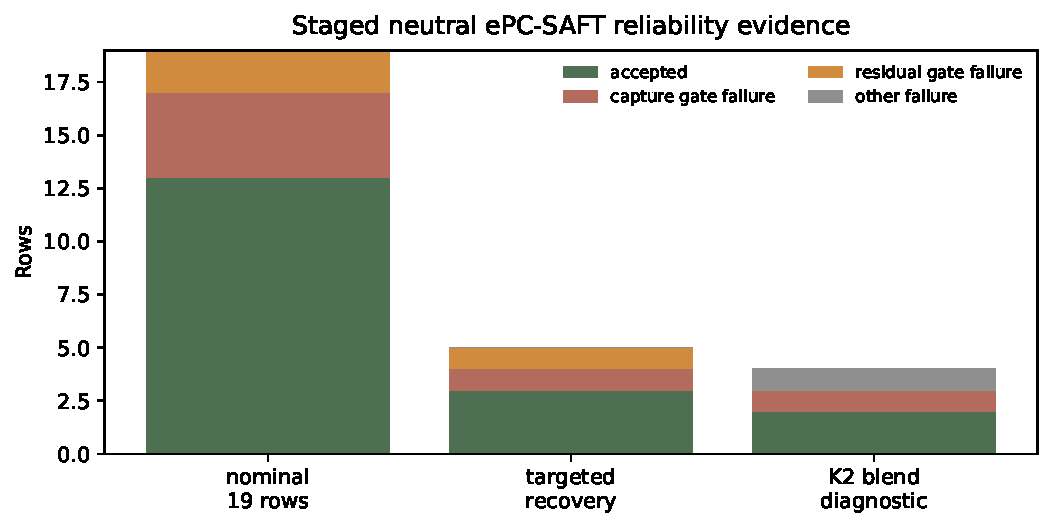
\includegraphics[width=0.76\textwidth]{figures/staged-epcsaft-reliability.pdf}
            \caption{Staged neutral ePC-SAFT reliability evidence. Accepted rows, capture-gate failures, residual-gate failures, and other failures are separated so the thermodynamic sensitivity lane is not overclaimed.}
            \label{fig:staged-epcsaft-reliability}
        \end{figure}

        \subsubsection*{Model Adequacy}
        A run is considered useful for validation only when numerical convergence and physical adequacy are both satisfied. Solver success alone is not enough. For one-bed C cases, adequacy requires a successful solve, finite boundary residuals, and reported capture and temperature-profile errors because measured temperature taps are available. For staged legacy K rows, adequacy is currently based on capture error, boundary residual, bed/intercooler metadata, and explicit caveats because the packaged K-row table does not include the same temperature tap data. Recovery rows and ePC-SAFT diagnostic rows are retained because they explain failure modes and plausible settings, but they are not used to claim broad predictive accuracy.

        Table~\ref{tab:case3c-epcsaft-pressure-state-smoke} reports the pressure-state ePC-SAFT smoke result for Case 3C after adding density-guess reuse to the MEA-side adapter. The density is not specified as the thermodynamic state variable; the previous converged molar density is passed only as an initial guess for the package's internal pressure-density solve. The ionic SSM/Born lane is therefore no longer a large runtime outlier in this smoke test, but it remains a diagnostic thermodynamic lane rather than primary staged validation.

        \begin{table}
            \centering
            \scriptsize
            \caption{Case 3C pressure-state thermodynamic smoke test for Henry-law, neutral ePC-SAFT, and six-species ionic ePC-SAFT lanes.}
            \label{tab:case3c-epcsaft-pressure-state-smoke}
            \renewcommand{\arraystretch}{1.2}
            \resizebox{\textwidth}{!}{%
            \begin{tabular}{lcccccc}
                \toprule
                \textbf{Thermo model} & \textbf{Success} & \textbf{Runtime (s)} & \textbf{Capture (\%)} & \textbf{Capture error (\%)} & \textbf{Temp. RMSE (K)} & \textbf{State time (s)} \\
                \midrule
                Henry-law baseline & Yes & 5.95 & 89.40 & -0.10 & 3.94 & 0.00 \\
                Neutral ePC-SAFT & Yes & 5.92 & 89.70 & 0.20 & 3.97 & 0.50 \\
                Ionic ePC-SAFT, SSM/Born & Yes & 6.15 & 89.83 & 0.33 & 3.97 & 0.34 \\
                \bottomrule
            \end{tabular}%
            }
        \end{table}

        Table~\ref{tab:staged-epcsaft-recovery-probe} summarizes the targeted recovery probe for staged neutral ePC-SAFT rows that failed the nominal diagnostic settings. K4 and K9 are recovered by moving the initial capture branch toward the measured capture level, and K23 is recovered when the inter-stage liquid cooling reset is weakened. K2 remains a large capture-error failure, and K19 remains a boundary-residual failure. These rows are therefore reported as solver-diagnostic evidence, not as a replacement for a global ePC-SAFT validation set.

        \begin{table}
            \centering
            \scriptsize
            \caption{Targeted staged neutral ePC-SAFT recovery probe for the nominal failed diagnostic rows.}
            \label{tab:staged-epcsaft-recovery-probe}
            \renewcommand{\arraystretch}{1.2}
            \begin{tabular}{lcccl}
                \toprule
                \textbf{Case} & \textbf{Accepted} & \textbf{Capture error (\%)} & \textbf{Boundary residual} & \textbf{Recovery setting} \\
                \midrule
                K2 & No & -55.96 & $1.00\times10^{-10}$ & capture guess 95, intercooler strength 0.25 \\
                K4 & Yes & 4.89 & $1.00\times10^{-10}$ & capture guess 78 \\
                K9 & Yes & 4.58 & $1.00\times10^{-10}$ & capture guess 55 \\
                K19 & No & 1.79 & $1.00\times10^{2}$ & capture guess 99 \\
                K23 & Yes & -4.10 & $8.05\times10^{-6}$ & capture guess 99, intercooler strength 0.25 \\
                \bottomrule
            \end{tabular}
        \end{table}

        Table~\ref{tab:staged-epcsaft-k2-blend-probe} reports the follow-on K2 thermodynamic continuation diagnostic. The blend parameter is applied only to the fugacity values returned by the thermodynamic driving-force adapter: zero corresponds to the Henry-law fugacity lane and one corresponds to the full neutral ePC-SAFT fugacity lane. The K2 row is accepted at blends of 0.50 and 0.75, and the 0.90 row reaches the capture and residual targets but is retained as a failed row because it exceeded the runtime cap. At blend 1.00, the same case returns to the zero-capture branch. This result supports a narrower interpretation of the staged ePC-SAFT limitation: K2 is not simply missing a high-capture initialization, but remains sensitive to the full neutral ePC-SAFT endpoint used for the CO$_2$ driving force.

        \begin{table}
            \centering
            \scriptsize
            \caption{K2 staged neutral ePC-SAFT fugacity-blend diagnostic.}
            \label{tab:staged-epcsaft-k2-blend-probe}
            \renewcommand{\arraystretch}{1.2}
            \begin{tabular}{ccccl}
                \toprule
                \textbf{Blend} & \textbf{Accepted} & \textbf{Capture error (\%)} & \textbf{Boundary residual} & \textbf{Status} \\
                \midrule
                0.50 & Yes & 0.51 & $8.68\times10^{-4}$ & partial blend accepted \\
                0.75 & Yes & 0.51 & $3.44\times10^{-2}$ & partial blend accepted \\
                0.90 & No & 0.51 & $1.01\times10^{-10}$ & timeout, low-residual final iterate \\
                1.00 & No & -99.49 & $3.03\times10^{-4}$ & full endpoint, zero-capture branch \\
                \bottomrule
            \end{tabular}
        \end{table}

        The selected generated temperature-profile PNG files are included in Figure~\ref{fig:generated-temperature-profiles}. These profiles are intentionally presented with the exact thermodynamic lane identified in the caption so that profile agreement, capture agreement, and solver convergence can be evaluated separately.

        \subsubsection*{Remaining Benchmark Scope}
        The present artifacts support the benchmark contribution, but they should not be interpreted as full predictive validation across every NCCC condition. The K6, K7, K8, and K20 Henry-law recovery rows require high mass-transfer factors, suppressed intercooler reset strength, or large guard counts, so they are retained as diagnostic and sensitivity evidence rather than primary validation. The staged neutral ePC-SAFT K2, K19, and K22 rows remain unresolved at the full fugacity endpoint under the current acceptance gates, and the K2 blend diagnostic indicates a branch-selection and thermodynamic-continuation limitation rather than a simple missing initial guess. Stronger predictive claims should be deferred until a documented global calibration or expanded thermodynamic model removes those case-specific recovery settings and is validated against additional pilot campaigns.
